% \DeclareDocumentMetadata {lang=en-US}

% xmp metadata for pdf
% Originally used \usepackage[a-2a]{pdfx}
% \usepackage{hyperxmp} replaced it
% \RequirePackage{pdfmanagement-testphase} replaced it
% \PassOptionsToPackage{enable-debug,check-declarations}{expl3} broke with version 0.9 of tagpdf
% \ExplSyntaxOn no need for these 3 lines because metadata can handle it
% \pdfmanagement_add:nnn{Catalog}{Lang}{(enUS)} enUS is wrong, should be en-US
% \ExplSyntaxOff

\documentclass[11pt,
  english,
  letterpaper,
]{article}
\usepackage{sa4ss}
\usepackage{amsmath,amssymb,array}
\usepackage{booktabs}

% From tagged-template.latex
\usepackage{lmodern}
\usepackage{ifxetex,ifluatex}
\ifnum 0\ifxetex 1\fi\ifluatex 1\fi=0 % if pdftex
  \usepackage[T1]{fontenc}
  \usepackage[utf8]{inputenc}
  \usepackage{textcomp} % provide euro and other symbols
\else % if luatex or xetex
  \usepackage{unicode-math}
  \defaultfontfeatures{Scale=MatchLowercase}
  \defaultfontfeatures[\rmfamily]{Ligatures=TeX,Scale=1}
\fi

% Use upquote if available, for straight quotes in verbatim environments
\IfFileExists{upquote.sty}{\usepackage{upquote}}{}
\IfFileExists{microtype.sty}{% use microtype if available
  \usepackage[]{microtype}
  \UseMicrotypeSet[protrusion]{basicmath} % disable protrusion for tt fonts
}{}
\makeatletter
\@ifundefined{KOMAClassName}{% if non-KOMA class
  \IfFileExists{parskip.sty}{%
    \usepackage{parskip}
  }{% else
    \setlength{\parindent}{0pt}
    \setlength{\parskip}{6pt plus 2pt minus 1pt}}
}{% if KOMA class
  \KOMAoptions{parskip=half}}
\makeatother
\usepackage{xcolor}
\IfFileExists{xurl.sty}{\usepackage{xurl}}{} % add URL line breaks if available
\hypersetup{
  pdftitle={Status of Black Rockfish (Sebastes melanops) off Oregon and federal waters in 2023},
  pdflang={en},
  hidelinks,
  pdfcreator={LaTeX via pandoc}}
\urlstyle{same} % disable monospaced font for URLs
\usepackage{longtable}
% Correct order of tables after \paragraph or \subparagraph
\usepackage{etoolbox}
\makeatletter
\patchcmd\longtable{\par}{\if@noskipsec\mbox{}\fi\par}{}{}
\makeatother
% Allow footnotes in longtable head/foot
\IfFileExists{footnotehyper.sty}{\usepackage{footnotehyper}}{\usepackage{footnote}}
\makesavenoteenv{longtable}
\usepackage{graphicx}
\makeatletter
\def\maxwidth{\ifdim\Gin@nat@width>\linewidth\linewidth\else\Gin@nat@width\fi}
\def\maxheight{\ifdim\Gin@nat@height>\textheight\textheight\else\Gin@nat@height\fi}
\makeatother
% Scale images if necessary, so that they will not overflow the page
% margins by default, and it is still possible to overwrite the defaults
% using explicit options in \includegraphics[width, height, ...]{}
\setkeys{Gin}{width=\maxwidth,height=\maxheight,keepaspectratio}
% Set default figure placement to htbp
\makeatletter
\def\fps@figure{htbp}
\makeatother
\setlength{\emergencystretch}{3em} % prevent overfull lines
\providecommand{\tightlist}{%
  \setlength{\itemsep}{0pt}\setlength{\parskip}{0pt}}
\setcounter{secnumdepth}{5}
\ifxetex
  % Load polyglossia as late as possible: uses bidi with RTL langages (e.g. Hebrew, Arabic)
  \usepackage{polyglossia}
  \setmainlanguage[]{}
\else
  \usepackage[shorthands=off,main=english]{babel}
\fi

%Define cslreferences environment, required by pandoc 2.8
%https://github.com/rstudio/rmarkdown/issues/1649
\newlength{\csllabelwidth}
\setlength{\csllabelwidth}{3em}
\newlength{\cslhangindent}
\setlength{\cslhangindent}{1.5em}
% for Pandoc 2.8 to 2.10.1
\newenvironment{cslreferences}%
  {}%
  {\par}
% For Pandoc 2.11+
\newenvironment{CSLReferences}[2] % #1 hanging-ident, #2 entry spacing
 {% don't indent paragraphs
  \setlength{\parindent}{0pt}
  % turn on hanging indent if param 1 is 1
  \ifodd #1 \everypar{\setlength{\hangindent}{\cslhangindent}}\ignorespaces\fi
  % set entry spacing
  \ifnum #2 > 0
  \setlength{\parskip}{#2\baselineskip}
  \fi
 }%
 {}
\usepackage{calc}  % for \widthof, \maxof in minipage
\newcommand{\CSLBlock}[1]{#1\hfill\break}
\newcommand{\CSLLeftMargin}[1]{\parbox[t]{\csllabelwidth}{#1}}
\newcommand{\CSLRightInline}[1]{\parbox[t]{\linewidth - \csllabelwidth}{#1}\break}
\newcommand{\CSLIndent}[1]{\hspace{\cslhangindent}#1}


\providecommand{\tightlist}{%
  \setlength{\itemsep}{0pt}\setlength{\parskip}{0pt}}


\date{}
\newcommand{\trTitle}{Status of Black Rockfish (\emph{Sebastes melanops}) off Oregon and federal waters in 2023}
\newcommand{\trYear}{2022}
\newcommand{\trMonth}{December}
\newcommand{\trAuthsLong}{truetrue}
\newcommand{\trAuthsBack}{Cope, J.M., A.D. Whitman}
\newcommand{\trCitation}{
\begin{hangparas}{1em}{1}
\trAuthsBack{}. \trYear{}. \trTitle{}. \glsentrylong{pfmc}, Portland, Oregon. \pageref{LastPage}{}\,p.
\end{hangparas}}

\begin{document}

%%%%% Frontmatter %%%%%

% Footnote symbols in front matter
\renewcommand*{\thefootnote}{\fnsymbol{footnote}}

\small
\thispagestyle{empty}
\pagenumbering{roman}
\noindent
\begin{center}
\title{Status of Black Rockfish (\emph{Sebastes melanops}) off Oregon and federal waters in 2023}
% \textnormal{\MakeTextUppercase{\trTitle{}}}
\vspace{1.5cm}
{\Large\textbf\newline{Status of Black Rockfish (\emph{Sebastes melanops}) off Oregon and federal waters in 2023}}
\vfill
by\\
Jason M. Cope\textsuperscript{1}\\
Alison D. Whitman\textsuperscript{2}\vfill
\textsuperscript{1}Northwest Fisheries Science Center, U.S. Department of Commerce, National Oceanic and Atmospheric Administration, National Marine Fisheries Service, 2725 Montlake Boulevard East, Seattle, Washington 98112\\
\textsuperscript{2}Oregon Department of Fish and Wildlife, 2040 Southeast Marine Science Drive, Newport, Oregon 97365\vfill
\trMonth{} \trYear{}
\end{center}
\clearpage

% Fourth page: Colophon
\thispagestyle{empty}
\vspace*{\fill}
\begin{center}
\copyright{} \glsentrylong{pfmc}, \trYear{}\\
\end{center}
\par
\bigskip
\noindent
Correct citation for this publication:
\bigskip
\par
\trCitation{}
\clearpage

% Add TOC to pdf bookmarks (clickable pdf)
\pdfbookmark[1]{\contentsname}{toc}

% Table of contents page, lists of figures and tables
\tableofcontents\clearpage
\label{TRlastRoman}
\clearpage

% Table of contents
\newpage
\thispagestyle{empty} % to remove page number

% Settings for the main document
\pagenumbering{arabic}  % Regular page numbers
\pagestyle{plain}  % No page number on first page of main document, use 'empty'
\renewcommand*{\thefootnote}{\arabic{footnote}}  % Back to numeric footnotes
\setcounter{footnote}{0}  % And start at 1
\renewcommand{\headrulewidth}{0.5pt}
\renewcommand{\footrulewidth}{0.5pt}
%\pagestyle{fancy}\fancyhead[c]{Draft: Do not cite or circulate}

\newcommand{\lt}{\ensuremath <}
\newcommand{\gt}{\ensuremath >}

\pagebreak
\pagenumbering{roman}
\setcounter{page}{1}

\renewcommand{\thetable}{\roman{table}}
\renewcommand{\thefigure}{\roman{figure}}

\setlength\parskip{0.5em plus 0.1em minus 0.2em}

\hypertarget{executive-summary}{%
\section*{Executive summary}\label{executive-summary}}
\addcontentsline{toc}{section}{Executive summary}

\hypertarget{stock}{%
\subsection*{Stock}\label{stock}}
\addcontentsline{toc}{subsection}{Stock}

The assessments described in this document apply to the black rockfish (\emph{Sebastes melanops}) stocks that reside in the waters from Point Conception (34\textdegree27' N latitude) in the south to the U.S. boundary with Canada (approximately 48\textdegree30' N latitude). Following the consensus recommendations from a preliminary stock assessment workshop in April 2015 (PFMC 2015), the stock assessment team (STAT) decided to prepare separate geographic stock assessments that are spatially stratified with boundaries at the CA/OR border (42\textdegree00' N latitude) and OR/WA border (46\textdegree16' N latitude).

Black rockfish are also caught from the waters off British Columbia and Alaska, but there have not been any formal assessments of stock status for those areas.

\hypertarget{catches}{%
\subsection*{Catches}\label{catches}}
\addcontentsline{toc}{subsection}{Catches}

Black rockfish are caught by a wide variety of gear types and in recent decades have been a very important target species for recreational charter-boats and private sport anglers in Washington and Oregon, and to a lesser extent in California. In recent years the recreational fishery has accounted for most of the black rockfish catches (Figure ES-1 to Figure ES-3). Black rockfish can also be an important component of nearshore commercial fisheries, either as incidental catch by the troll fishery for salmon or as directed catch by jig fisheries for groundfish. Further, in California and Oregon there are nearshore fisheries that catch and sell fish live for the restaurant trade. Washington closed nearshore commercial fisheries in state water in late 1990s and never allowed the live-fish fishery to develop. In all states there have been almost no trawl-caught landings of black rockfish in recent years (Table ES-1), but trawl landings in the past were substantial (Figure ES-1 to Figure ES-3).

Detailed reports of commercial landings of black rockfish are generally unavailable prior to 1981, when the Pacific Fishery Information Network (PacFIN) database began. The catch series prior to 1981 for these assessments were derived by applying available estimates or assumed values for the proportion of black rockfish landings in reported landings of rockfish. Observer data, which are available only for the past decade, indicate low levels of discarding of black rockfish, generally less than 2\% of total catch.

Because of their nearshore distribution and low abundance compared to other rockfish species, black rockfish are unlikely to have ever comprised a large percentage of rockfish landings, but it seems quite certain that they have been more than a trivial component for many years. Black rockfish were one of only four rockfish species mentioned by scientific name in reports of rockfish landings in Oregon during the 1940s, and they were one of only six rockfish species mentioned by scientific name in reports of rockfish landings in California during the same period. Mentions of black rockfish extend back before the year 1900 in Washington.

\hypertarget{data-and-assessment}{%
\subsection*{Data and assessment}\label{data-and-assessment}}
\addcontentsline{toc}{subsection}{Data and assessment}

The last stock assessments for black rockfish were conducted in 2007 for areas north and south of Cape Falcon (45\textdegree46' North latitude). The current assessments assume three areas instead of two, delineated by the state lines as was agreed upon at a pre-assessment and data workshop in March 2015. The prior assessments used Stock Synthesis 2, while the current assessments use Stock Synthesis

\begin{verbatim}
[1] "3.30.20.00"
\end{verbatim}

. The Washington base assessment includes a dockside and tag-based CPUE series, but does not include the abundance estimate time series from that same tagging study which was included in the last assessment due to too many violations in the assumptions of abundance estimation. The same two commercial and single recreational fleets are used as in the last assessment for Washington. The Oregon assessment has three commercial fleets and two recreational fleets, while using five surveys and an additional research study for biological compositions. California also has three commercial fleets and 1 recreational fleet with three surveys of abundance, all based on recreational fisheries. All area models include age data as conditional age at lengths. Length compositions are also included in all models.

\hypertarget{stock-biomass-and-dynamics}{%
\subsection*{Stock biomass and dynamics}\label{stock-biomass-and-dynamics}}
\addcontentsline{toc}{subsection}{Stock biomass and dynamics}

Spawning stock outputs are all at or above limit reference points (Table ES-2. Only California shows declines significantly below this reference point at any point in the time series. California and Washington stocks show a declining population through most of the 20th Century, with stronger declines in the 1980s, and recoveries beginning in the mid-1990s. Oregon stocks follow this pattern, but with a decline in the most recent period. California (33\%) is below the target biomass reference point with an increasing biomass trend (Figures ES-4 and ES-5). The Oregon stock dropped after the quick ramp up of catches in the late 1970s and continued a steady decline until around year 2000, settling in at a stock status around 60\% of initial conditions. The Washington stock, currently 43\%, dropped below the target biomass by in the early 1980s, then risen above since the late 1990s and has fluctuated above that point through 2014 (Figures ES-8 and ES-9).

\hypertarget{recruitment}{%
\subsection*{Recruitment}\label{recruitment}}
\addcontentsline{toc}{subsection}{Recruitment}

The California model shows a few extraordinarily high recruitment events that are supported by the length composition data, index data and on-the-water reports (Table ES-3; Figure ES-10). Oregon recruitment is highly uncertain (Table ES-3; Figure ES11). Washington recruitment is dynamic, but also shows the most informed recruitment time series, which is consistent with the extent of length and age compositions available to that assessment (Table ES-3; Figure ES12). Both California and Washington support elevated recruitment in the late 2000s.

\hypertarget{exploitation-status}{%
\subsection*{Exploitation status}\label{exploitation-status}}
\addcontentsline{toc}{subsection}{Exploitation status}

California and Washington models indicate that current fishing practices are near or above the SPR rate fishing intensity target, while the Oregon model is quite a bit above the target (table ES-4, compare to SPR=0.5; Figure ES-13 to Figure ES-18), though the steepness value (0.773) indicates a much lower value of SPR for sustainable removals. Fishing rates have been above the target in California in nearly all years since the 1980s, but have dropped considerably in recent years. Oregon fishing rates have been consistently high in recent years. Washington shows a dramatic decline in fishing intensity since the late 1990s and has fluctuated mostly below the target since.

\hypertarget{ecosystem-considerations}{%
\subsection*{Ecosystem considerations}\label{ecosystem-considerations}}
\addcontentsline{toc}{subsection}{Ecosystem considerations}

Ecosystem considerations were not explicitly included in these models, though growth deviations were considered in the Washington model. While no mechanisms have been put forth for these time-varying changes in growth, an environmental component is possible. Limited data in Oregon and California also suggest the possibility that growth has changed over time.

\hypertarget{reference-points}{%
\subsection*{Reference points}\label{reference-points}}
\addcontentsline{toc}{subsection}{Reference points}

Reference points were based on the rockfish FMSY proxy (SPR50\%), target relative biomass (40\%) and model-estimated selectivity for each fleet. California is below the target biomass reference point, but above the limit reference biomass (25\%). Oregon is well above the target biomass. Washington relative biomass is above the target biomass. California and Washington yield values are lower than the previous assessment for similar reference points due to lower overall natural mortality values (Table ES-5). The proxy MSY values of management quantities are the most conservative compared to the estimated MSY and MSY relative to 40\% biomass for both California and Washington (Table ES-5). The equilibrium estimates of yield relative to biomass are provided in Figure ES-19 to Figure ES-21.

\hypertarget{management-performance}{%
\subsection*{Management performance}\label{management-performance}}
\addcontentsline{toc}{subsection}{Management performance}

Removals have been below the equivalent ABC-ACL since the prior assessment (Table ES-6), but those specified ABCs from the 2007 assessments are higher than those coming from the current assessment models. Removals over the last few years have or may have exceeded the newly estimated ABC-ACL values in some years. The differences in the treatment of natural mortality between the previous and current assessments are the biggest reason for this discrepancy.

\hypertarget{unresolved-problems-and-major-uncertainties}{%
\subsection*{Unresolved problems and major uncertainties}\label{unresolved-problems-and-major-uncertainties}}
\addcontentsline{toc}{subsection}{Unresolved problems and major uncertainties}

The most significant uncertainty for all models is the treatment and value of natural mortality and the form of fleet selectivity (e.g., length-based asymptotic vs.~age-based dome-shaped selectivity). Data-driven selection between the extreme ``kill'' (using a ramping of M) or ``hide'' hypotheses are not currently resolvable. The current California and Washington base models instead use a form of the ``kill'' hypothesis by not implementing the age-based selectivity (``hide'' hypothesis) and estimating female and male natural mortality, thus avoiding a fixing natural mortality as was necessary in the Oregon model. The Oregon model also contained a step in female natural mortality, a specification not used in the California or Washington models. Another important issue is the highly uncertain historical time-series of removals in all states, which needs further consideration. The development of fishery-dependent indices of abundance still requires further attention. Steepness, while fixed, is still highly uncertain for rockfishes and currently is mismatched to the MSY proxy. And while the steepness profile shows low sensitivity in several derived quantities, steepness strongly defines the yield capacity of stocks, and therefore could cause major uncertainty in the recommended management quantities. Stock structure and its relationship to the current political/management boundaries are also not fully understood, both within U.S. jurisdiction and between the U.S. and Canada. While this is a common challenge faced in most west coast stock assessments, further improvement on this topic will likely rely on black rockfish-specific data.

\hypertarget{decision-table-and-projections}{%
\subsection*{Decision table and projections}\label{decision-table-and-projections}}
\addcontentsline{toc}{subsection}{Decision table and projections}

Black rockfish assessments for California and Washington have a preliminary distinction as category 1 stock assessments, thus harvest projections and decision tables are based on using P\emph{=0.45 and sigma = 0.36, resulting in a multiplier on the OFL of 0.956. The Oregon black rockfish assessment is a category 2 assessment, with a P}=0.45 and sigma = 0.72 with a multiplier of 0.913 applied to the OFL. These multipliers are also combined with the rockfish MSY proxy of FSPR=50\% MSY and the 40-10 harvest control rule to calculate OFLs, ABCs and ACLs. Projections for each state are provided in Table ES-7 to Table ES-9.

Uncertainty in management quantities for the base model of each state was characterized by exploring various model specifications in a decision table. Initial exploration included natural mortality and steepness values, and uncertainty in historical trawl catches for the WA and CA models. OR explored the scale factor coming from the value of the tagging catchability (Q) parameter, as well as M values. For the CA and WA models, there was very little sensitivity to steepness and trawl catches, but natural mortality produced sensitive results of predicted population scale and status. Discussion with the STAR panel resulted in high and low states of nature +/- 0.03 from the base case natural mortality values for females and males. High and low catch streams (rows) were determined by the forecasts, as described above, for each state of nature. Thus the low catch stream is based on the forecast from the low state of nature. The OR model demonstrated little sensitivity to M, but high sensitivity to the tagging survey Q. High and low states of nature, respectively, were based on a fixed tag of Q = 0.125 and Q estimated by the model. Resultant decision tables are provided in Table ES-10 to Table ES-12.

\hypertarget{scientific-uncertainty}{%
\subsection*{Scientific uncertainty}\label{scientific-uncertainty}}
\addcontentsline{toc}{subsection}{Scientific uncertainty}

The model-estimated uncertainty around the 2015 spawning biomass was \(\sigma\) = 0.01 and the uncertainty around the OFL was \(\sigma\) = 0.01. This is likely an underestimate of overall uncertainty because of the necessity to fix some parameters such as steepness, as well as a lack of explicit incorporation of model structural uncertainty.

\hypertarget{research-and-data-needs}{%
\subsection*{Research and data needs}\label{research-and-data-needs}}
\addcontentsline{toc}{subsection}{Research and data needs}

Recommended avenues for research to help improve future black rockfish stock assessments:

\begin{enumerate}
\def\labelenumi{\arabic{enumi}.}
\tightlist
\item
  Further investigation into the movement and behavior of older (\textgreater{} age 10) females to reconcile their absence in fisheries data. If the females are currently inaccessible to fishing gear, can we find where they are?
\item
  Appropriate natural mortality values for females and males. This will help resolve the extent to which dome-shaped age-based selectivity may be occurring for each.
\item
  All states need improved historical catch reconstructions. The trawl fishery catches in particular require particular attention. Given the huge historical removals of that fleet in each state, the assessment is very sensitive to the assumed functional form of selectivity. A synoptic catch reconstruction is recommended, where states work together to resolve cross-state catch issues as well as standardize the approach to catch recommendations.
\item
  Identifying stanzas or periods of uncertainty in the historical catch series will aid in the exploration of catch uncertainty in future assessment sensitivity runs.
\item
  The ODFW tagging study off Newport should be continued and expanded to other areas. To provide better prior information on the spatial distribution of the black rockfish stock, further work should be conducted to map the extent of black rockfish habitat and the densities of black rockfish residing there.
\item
  An independent nearshore survey should be supported in all states to avoid the reliance on fishery-based CPUE indices.
\item
  Stock structure for black rockfish is a complicated topic that needs further analysis. How this is determined (e.g., exploitation history, genetics, life history variability, biogeography, etc.) and what this means for management units needs to be further refined. This is a general issue for all nearshore stocks that likely have significant and small scale stock structure among and within states, but limited data collections to support small-scale management.
\end{enumerate}

\vspace{500cm}

\pagebreak
\setlength{\parskip}{5mm plus1mm minus1mm}
\pagenumbering{arabic}
\setcounter{page}{1}
\renewcommand{\thefigure}{\arabic{figure}}
\renewcommand{\thetable}{\arabic{table}}
\setcounter{table}{0}
\setcounter{figure}{0}

\hypertarget{introduction}{%
\section{Introduction}\label{introduction}}

\hypertarget{basic-information}{%
\subsection{Basic Information}\label{basic-information}}

Black Rockfish (\emph{Sebastes melanops}) are an important component of the recreational fisheries in the nearshore waters off central and northern California, Oregon, and Washington, as well as the non-trawl commercial fisheries in California and Oregon. They range as far north as Amchitka and Kodiak islands in Alaska and are considered uncommon south of central California (Love et al.~2002).

A previous assessment of Black Rockfish off Oregon and California (Ralston and Dick 2003) reviewed the evidence supporting genetic stock structure for Black Rockfish and other rockfish off the U.S. West Coast and concluded that the Oregon and California populations of Black Rockfish are probably not genetically heterogeneous. That assessment treated the Black Rockfish off California and Oregon as a unit stock. Previous assessments of Black Rockfish off Washington (Wallace et al.~1999, 2007) describe a study of coastal Black Rockfish genetic structure using 10 sampled sites collected from northern California to southern British Columbia t 1995-97. Results of that study support the notion of separate genetic stocks north and south of Cape Falcon. However, a later study (Baker 1999) of Black Rockfish collected from eight sites along the northern Oregon coast concluded that Black Rockfish from north and south of Cape Falcon were genetically very similar.

Although a stock boundary line at the Columbia River seems reasonable for Black Rockfish, both because it is a state fishery management boundary and because the Columbia River plume is likely to be a natural barrier to the north-south exchange of Black Rockfish adults and larvae, the 2007 assessment of Black Rockfish off Oregon and California (Sampson 2007) differed slightly from Ralston and Dick (2003) in placing the northern boundary at Cape Falcon rather than at the Columbia River. The boundary was changed to avoid overlap with the separate northern assessment (Wallace et al.~2007) and to simplify the process of assembling historical commercial landings data, which are largely available in terms of Pacific Marine Fisheries Commission (PMFC) statistical areas. The northern boundary of PMFC Area 2C is at Cape Falcon (Figure 1). Given the spatial resolution of the historical commercial fishery data, it is very problematic to estimate the catch of Black Rockfish taken north of Cape Falcon but south of the Columbia River.

During a preliminary workshop in April 2015 (PFMC 2015), to discuss approaches for assessing Black Rockfish, China rockfish (\emph{S. nebulosus}), and kelp greenling (\emph{Hexagrammos decagrammus}), it was agreed that the assessments for these nearshore species should at a minimum be spatially stratified with boundaries at the CA/OR border (42\textdegree00' N latitude) and the OR/WA border (46\textdegree16' N latitude). Such a spatial stratification would be consistent with two ideas: (a) these nearshore species do not exhibit much adult movement and (b) exploitation and management histories have varied significantly among the three states. Together these features would likely create appreciable state-to-state differences in age composition for each of the three species. Stock assessment teams were advised that they could use geographic strata that were finer than the state level if there were data to support such an approach (Figure 1).

At the same nearshore stock assessment workshop, it was agreed that recreational catch histories for the stocks of Black Rockfish should be assembled on the basis of port of landing rather than location of fish capture, even though fishing vessels landing their catches into a port in one state might have captured fish in waters off a neighboring state.

Accounting for location of capture is very problematic for recreationally caught fish and for commercial catches taken with non-trawl types of gear (e.g., hook-and-line), for which there are no or very limited logbooks that report fishing location. For these regional assessments the commercially caught Black Rockfish were apportioned to assessment region based on the port of landing, with the exception of trawl caught fish landed into Astoria, OR. Most of these fish were assumed to have been caught off Washington and most of the trawl landings into Astoria were therefore included with the catch history for the Washington assessment region. Details are provided below in Section 2.1.1.1 The PacFIN Era (1981 to 2014).

\hypertarget{life-history}{%
\subsection{Life History}\label{life-history}}

Adults tend to occur in schools over rocky structure at depths less than 40 fathoms, and sometimes feed actively on or near the surface. They feed on a wide variety of prey including zooplankton, krill, mysids, sand lance, and juvenile rockfish (Love 1969), and are subject to predation by lingcod and marine mammals.

Although tagging studies have documented some individuals moving long distances (several hundreds of miles), the vast majority of recaptured individuals were found close to the areas of initial capture and tagging (Culver 1987; Ayres 1988; Starr and Green 2007; Wallace et al.~2010). Results from a 2004-05 study off Newport, OR of 42 Black Rockfish implanted with acoustic tags indicated that all but seven fish remained within range of a 3 x 5 km array of acoustic receivers during one full year of monitoring and had relatively small home ranges that did not vary seasonally (Parker et al.~2007). Green and Starr (2011) report similar findings from a study in Carmel Bay, CA of 23 acoustically tagged Black Rockfish. The extensive Washington state tagging study also supported low movements for most individuals, with some exceptional movements recorded (Wallace et al.~2010).

Like all members of the genus Sebastes, Black Rockfish have internal fertilization and bear live young approximately two months after insemination. Black Rockfish are quite fecund, with a six-year-old female annually producing about 300,000 embryos and a 16-year-old producing about 950,000 embryos (Bobko and Berkeley 2004). Recent studies have demonstrated that the relative number and quality of larvae increase with age in female Black Rockfish (Berkeley et al.~2004; Hixon et al.~2014). Parturition of larvae occurs during winter (Wyllie-Echeverria 1987) and larvae and small juveniles are pelagic for several months to a year (Boehlert and Yoklavich 1983). Settlement occurs in estuaries, tide-pools, and in the nearshore at depths less than 20 m (Stein and Hassler 1989).

Black Rockfish begin recruiting to nearshore fisheries at 3-4 years of age, corresponding to a fork length of about 25-30 cm, and 50\% of females attain maturity at about 6-8 years, corresponding to a fork length of about 38-42 cm. Adult female Black Rockfish grow 3-5 cm larger than males, with a few females attaining fork lengths greater than 55 cm.

\hypertarget{ecosystem-considerations-1}{%
\subsection{Ecosystem Considerations}\label{ecosystem-considerations-1}}

No formal ecosystem considerations have been made given the lack of data for such an undertaking. Differences in growth though time have been considered in the model specification in the Washington model. Though the mechanism is not specified, this could certainly be due to process error driven by environmental conditions.

\hypertarget{historical-and-current-fishery-information}{%
\subsection{Historical and Current Fishery Information}\label{historical-and-current-fishery-information}}

Black Rockfish are harvested by a wide variety of fishing methods including trawling, trolling, and hook-and-line fishing with jigs and long-lines. Although Black Rockfish have never been a dominant component of any commercial fisheries, they are important as incidental catch in the troll fishery for salmon and the troll and jig fisheries for groundfish. With the decline of salmon fishing opportunities in the late 1970s and early 1980s Black Rockfish became a vital target of marine recreational fisheries in Oregon and Washington, especially during periods of restricted or slack fishing for salmon, halibut, and tuna.

Black Rockfish are also an important component of the recreational fisheries in northern California but are of less significance south of Cape Mendocino due to their reduced prevalence compared to other species. Since 1990 annual recreational harvests of Black Rockfish have averaged 229.6 tons off California, 304.4 tons off Oregon, and 272.5 tons off Washington. Commercial annual harvests by non-trawl gear types during the same period averaged 44.6 tons in California, 62.0 tons in Oregon, and 14.7 tons in Washington. Harvests by trawl on average during this period have been less than 19.3 tons annually for all three states combined.

Removal histories have been a significant axis of uncertainty in the past assessments of Black Rockfish. Because of concerns about the effects of initial equilibrium assumptions on the level of depletion estimated in the preliminary base model, the 2003 Stock Assessment Review (STAR) panel worked with the Stock Assessment Team (STAT) to develop a catch history that avoided the need to assume historical catch and equilibrium conditions in the first year of the assessment. The assumed catch reconstruction began in 1946, ramping up from zero in 1945 and all prior years. In hindsight, this may not have been a good assumption, as indicated by the following text from Cleaver (1951) that describes catches of rockfish from 1941 to 1949 in Oregon.

``The rockfish are caught by otter trawl and long-line gear. The principal species caught by the otter trawl are the Black Rockfish (\emph{Sebastodes melanops}); green or yellowtail rockfish (\emph{S. flavidus}); red or orange rockfish (\emph{S. pinniger}); and rosefish (\emph{S. alutus}). The landings of rockfish (all species) rose rapidly during the war from 1,301,400 pounds in 1941 to a peak of over 17,000,000 in 1945. Subsequently the landings fell rapidly because of decreased demand and leveled off at about 4,000,000 per year in 1949.

Cleaver also states, in an introductory section on Bottom Fisheries, that the ``otter trawl fishery accounts for at least 95 percent by weight of the bottom fish landings.''

That Black Rockfish is one of only four species that Cleaver identifies as composing the large landings of rockfish in Oregon (most of which was actually taken off of Washington waters) during WWII suggests that Black Rockfish were not a trivial fraction of the large catches taken during the 1940s. One might also suppose that the otter trawl fishery took a large portion of the landings of Black Rockfish. Cleaver's statements are certainly at odds with the catch reconstruction developed in the previous assessments.

It seems that Black Rockfish were also landed in appreciable quantities in California during the 1940s. Black Rockfish was identified by scientific name as one of the ``half-dozen of the larger and more abundant species {[}that{]} make up over half of the annual California commercial poundage landed'' (Anon. 1949).

A major task for the 2007 assessments of Black Rockfish in was developing a plausible reconstruction of historical landings of Black Rockfish and exploring the consequences of those landings. For the current set of assessments catch histories from the past assessments have been reconsidered. Formal catch reconstructions have been conducted in California (Ralston et al.~2010) and Oregon (Karnowski et al.~2014), but even those relatively newer attempts were reconsidered in light of contributions from state agencies. For this assessment, Washington provided a first step in an approach to provide a reconstructed historical catch time series for a stock, something needed for all species in the state's waters.

\hypertarget{summary-of-management-history-and-performance}{%
\subsection{Summary of Management History and Performance}\label{summary-of-management-history-and-performance}}

Prior to 2000 the Pacific Fishery Management Council (PFMC or Council) managed the fishery for Black Rockfish as part of the Sebastes complex, with no separate Acceptable Biological Catch (ABC) or Optimum Yield (OY) for Black Rockfish. In 2000 the Council established an ABC of 1,200 mt for Black Rockfish caught north of Cape Mendocino (in the Eureka, Columbia, and Vancouver INPFC statistical areas), but left Black Rockfish south of Cape Mendocino as part of the ``other rockfish'' category. For 2001 through 2003 the ABC for Black Rockfish caught north of Cape Mendocino was 1,115 mt annually, and Black Rockfish south of Cape Mendocino remained part of the ``other rockfish'' category and without a separate ABC or OY.

Regulation of the Black Rockfish fisheries by the PFMC prior to 2004 was accomplished primarily by trip limits for commercial fisheries and bag limit restrictions for recreational fisheries, with different limits applying in different geographic regions (see Table 1 in Ralston and Dick, 2003). Some other important regulations include the following.

\begin{itemize}
\tightlist
\item
  1953: California prohibited trawling within three miles of shore.
\item
  1995: The commercial hook-and-line fishing in Washington state waters (0-3 miles) was closed to preserve recreational fishing opportunities and avoid localized depletion; the closure was extended to trawlers in 1999. Oregon established Black Rockfish management areas with reduced daily commercial fishery trip limits in area near ports with large recreational fisheries.
\item
  2000: Black Rockfish began to be managed by the Council as a minor nearshore species. Commercial trip limits were significantly reduced, with specific restrictions applying to Black Rockfish. California instituted seasonal closures for commercial and recreational fisheries inside 20 fathoms, reduced the bag limit for rockfish from 15 to 10 fish, and limited recreational gear to one line with three hooks.
\item
  2002: California adopted a Nearshore Fishery Management Plan and began more active management of nearshore fisheries including the use of seasonal, regional, and depth-specific closures. Oregon adopted an Interim Nearshore Fishery Management Plan in anticipation of increased pressure on nearshore stocks due to reduced fishing opportunities for groundfish in federal waters. Regulations included fishing-sector specific caps on retained harvests, set approximately at the levels attained in 2000.
\item
  2003: The Council established Rockfish Conservation Areas (RCAs) to control catches of overfished rockfish species, and large portions of the shelf were closed to fishing. Differential trip limits were applied north and south of a management boundary at 40\textdegree10' N. latitude for nearshore Sebastes species. Nearshore permittees in California became subject to depth restrictions consistent with the shoreward non-trawl RCA boundary. In California the commercial and recreational fisheries for rockfish were closed early.
\item
  In 2004 and 2005: the sport fishery in Oregon closed in September 2004 due to early attainment of the state's limit for sport-caught Black Rockfish. This was the first time that the sport rockfish fishery in Oregon had not been open all year. In 2005 it closed early again.
\item
  In 2008 the groundfish trawl fishery was closed in Washington from the seaward RCA boundary to the shore north of 48\textdegree10' N. latitude to address increased encounters with yelloweye rockfish and canary rockfish.
\end{itemize}

In recent years California, Oregon and Washington regulations for the marine sport fisheries, which has been the major source of mortality on Black Rockfish, have become quite complicated and variable through time. Tools for regulating the sport fishery include closed areas, depth restrictions, seasonal closures, and bag limits.

California had no recreational bag limit for rockfish until 1990 when a 15 fish per day per angler limit was implemented. In 2000 the limit was reduced to 10 fish per day for each angler's combined bag of rockfish, cabezon and greenling. The fishing season was year-round prior to 2000 and since then has been variable by state management area. There were no gear restrictions prior to 2000. In 2000 anglers were limited to fishing one line with three hooks. Since 2001 they have been restricted to one line with two hooks. There is no minimum size limit for Black Rockfish.

Oregon had no recreational bag limits for marine fishes until 1976 when the state established a 25-fish limit. In 1978 the state established a daily limit of 15 fish for each angler's combined bag of rockfish, cabezon and greenling, which stayed in effect until 1994 when the state established a 10-fish-per-angler daily bag limit specifically for Black Rockfish. Following the early closure of the fishing season for Black Rockfish in 2004, the daily bag limit for Black Rockfish was dropped to 5 fish at the start of 2005 but was increased in-season to 6 fish. The per-angler daily bag limit was 6 fish during 2006 and 2007, 5 fish at the start of 2008 and increased in-season to 6 fish, 6 fish at the start of 2009 and increased in-season to 7 fish where it has remained since.

The goal of Oregon's sport fishery management is to maintain year-round fishing opportunities. In-season adjustments to regulations can be made more restrictive or less restrictive, depending on circumstances and the prospects for early attainment of harvest caps. Seasonal depth restrictions (e.g., inside 30 fathoms April 1 to September 30) are one tool used regularly in recent years to control the fishery, driven largely by the need to avoid bycatch of the primary rebuilding species, canary rockfish and yelloweye rockfish.

Washington had a recreational daily bag limit for rockfish (all species) of 15 fish per day from 1961 to 1991, 12 fish per day from 1992 to 1994, and 10 fish per day from 1995 to 2015. The bag limit for blue rockfish plus Black Rockfish in Marine Area 4B (Neah Bay) has been 6 fish per day since 2010. Fishing seasons for groundfish species are structured to provide year-round fishing opportunities, if possible. Depth restrictions vary by state management area, being more restrictive in the north compared to the south due to higher encounter rates with overfished yelloweye rockfish and canary rockfish. There is no minimum size limit for Black Rockfish.

In 2004 the coastwide ABC established for Black Rockfish was based on the projected yields derived from separate northern (Wallace et al.~1999) and southern (Ralston and Dick 2003) stock assessments (Table 1). The northern assessment covered the Washington coast and the northernmost portion of Oregon, from Cape Falcon to the WA/OR border at the Columbia River. The southern assessment covered the entire Oregon coast and the California coastline north of Point Arena.

To account for the spatial overlap of the two assessment areas, 12\% of the projected yield from the northern assessment was transferred to the southern region when deriving the coastwide ABC and OY values of 1,315 mt for 2004. State-by-state harvest guidelines were established: 326 mt for California, 450 mt for Oregon, and 540 mt for Washington. A similar approach was taken in 2005 and 2006 and the OY for the area south of the Columbia River was apportioned to harvest guidelines for California and Oregon based on a 42:58 split. The basis for this apportionment is unclear was to support separate harvest guidelines for each state. The catches were apportioned by the average catch share by state in the 1985-2002 period (PFMC 2004).

In all years when there has been an OY specified for Black Rockfish the estimated catch has been less than the OY, except for 2003 when the estimated coastwide catch exceeded the ABC for north of Cape Mendocino. In 2003 the estimated coastwide catch exceeded the OY by 183 mt for the region north of Cape Mendocino, but 290 mt of this coastwide catch was recreational harvest taken south of Cape Mendocino.

\hypertarget{canadian-and-alaska-fisheries}{%
\subsection{Canadian and Alaska fisheries}\label{canadian-and-alaska-fisheries}}

Black Rockfish is a ``Non-Quota'' species in the Department of Fisheries and Oceans Management Plan, and is not formally assessed in nearshore Canada waters (DFO, 2014).

Stock assessments are not conducted for Black Rockfish stocks in Southeast Alaska or Central Alaska, and there is no concern for these stocks at this time, because the directed fisheries for Black Rockfish and pelagic shelf rockfish in these areas are small with reduced fishing effort in recent years. In the Westward region (Kodiak area) directed fisheries for Black Rockfish have been conservatively managed in the past, and a stock assessment program in this region is being developed based on acoustic techniques as an index of abundance with a goal of incorporating these data into an age-structured model in the future (Alaska Department of Fish and Wildlife, 2015).

\hypertarget{data}{%
\section{Data}\label{data}}

Data comprise the foundational components of stock assessment models. The decision to include or exclude particular data sources in an assessment model depends on many factors. These factors often include, but are not limited to, the way in which data were collected (e.g., measurement method and consistency); the spatial and temporal coverage of the data; the quantity of data available per desired sampling unit; the representativeness of the data to inform the modeled processes of importance; timing of when the data were provided; limitations imposed by the Terms of Reference; and the presence of an avenue for the inclusion of the data in the assessment model. Attributes associated with a data source can change through time, as can the applicability of the data source when different modeling approaches are explored (e.g., stock structure or time-varying processes). Therefore, the specific data sources included or excluded from this assessment should not necessarily constrain the selection of data sources applicable to future stock assessments for Black Rockfish. Even if a data source is not directly used in the stock assessment they can provide valuable insights into biology, fishery behavior, or localized dynamics.

Data from a wide range of programs were available for possible inclusion in the current assessment model. Descriptions of each data source included in the model (Figure \ref{fig:data-plot}) and sources that were explored but not included in the base model are provided below. Data that were excluded from the base model were explicitly explored during the development of this stock assessment or have not changed since their past exploration in a previous Black Rockfish stock assessment. In some cases, the inclusion of excluded data sources were explored through sensitivity analyses (see Section \ref{assessment-model}).

\hypertarget{fishery-dependent-data}{%
\subsection{Fishery-Dependent Data}\label{fishery-dependent-data}}

\hypertarget{fishery-independent-data}{%
\subsection{Fishery-Independent Data}\label{fishery-independent-data}}

\hypertarget{section}{%
\subsubsection{\texorpdfstring{\acrlong{s-aslope}}{}}\label{section}}

The \gls{s-aslope} operated during the months of October to November aboard the R/V \emph{Miller Freeman}. Partial survey coverage of the US west coast occurred during the years 1988-1996 and complete coverage (north of 34\textdegree 30\textquotesingle S) during the years 1997 and 1999-2001. Typically, only these four years that are seen as complete surveys are included in assessments.

\hypertarget{section-1}{%
\subsubsection{\texorpdfstring{\acrlong{s-ccfrp}}{}}\label{section-1}}

Since 2007, the \gls{s-ccfrp} has monitored several areas in California to evaluate the performance of \glspl{mpa} and understand nearshore fish populations (Wendt and Starr 2009; Starr et al. 2015). In 2017, the survey expanded beyond the four \Gls{mpa}s in central California (Año Nuevo, Point Lobos, Point Buchon, and Piedras Blancas) to include the entire California coast. Fish are collected by volunteer anglers aboard \glspl{cpfv} guided by one of the following academic institutions based on proximity to fishing location: Humboldt State University; Bodega Marine Laboratories; Moss Landing Marine Laboratories; Cal Poly San Luis Obispo; University of California, Santa Barbara; and Scripps Institution of Oceanography.

Surveys consist of fishing with hook-and-line gear for 30-45 minutes within randomly chosen 500 by 500 m grid cells within and outside \glspl{mpa}. Prior to 2017, all fish were measured for length and release or descended to depth; since then, some were sampled for otoliths and fin clips.

\hypertarget{section-2}{%
\subsubsection{\texorpdfstring{\acrlong{s-tri}}{}}\label{section-2}}

The \gls{s-tri} was first conducted by the \gls{afsc} in 1977, and the survey continued until 2004 (Weinberg et al. 2002). Its basic design was a series of equally-spaced east-to-west transects across the continential shelf from which searches for tows in a specific depth range were initiated. The survey design changed slightly over time. In general, all of the surveys were conducted in the mid summer through early fall. The 1977 survey was conducted from early July through late September. The surveys from 1980 through 1989 were conducted from mid-July to late September. The 1992 survey was conducted from mid July through early October. The 1995 survey was conducted from early June through late August. The 1998 survey was conducted from early June through early August. Finally, the 2001 and 2004 surveys were conducted from May to July.

Haul depths ranged from 91-457 m during the 1977 survey with no hauls shallower than 91 m. Due to haul performance issues and truncated sampling with respect to depth, the data from 1977 were omitted from this analysis. The surveys in 1980, 1983, and 1986 covered the US West Coast south to 36.8\textdegree N latitude and a depth range of 55-366 m. The surveys in 1989 and 1992 covered the same depth range but extended the southern range to 34.5\textdegree N (near Point Conception). From 1995 through 2004, the surveys covered the depth range 55-500 m and surveyed south to 34.5\textdegree N. In 2004, the final year of the \gls{s-tri} series, the \gls{nwfsc} \gls{fram} conducted the survey following similar protocols to earlier years.

\hypertarget{section-3}{%
\subsubsection{\texorpdfstring{\acrlong{s-wcgbt}}{}}\label{section-3}}

The \Gls{s-wcgbt} is based on a random-grid design; covering the coastal waters from a depth of 55-1,280 m (Bradburn, Keller, and Horness 2011). This design generally uses four industry-chartered vessels per year assigned to a roughly equal number of randomly selected grid cells and divided into two `passes' of the coast. Two vessels fish from north to south during each pass between late May to early October. This design therefore incorporates both vessel-to-vessel differences in catchability, as well as variance associated with selecting a relatively small number (approximately 700) of possible cells from a very large set of possible cells spread from the Mexican to the Canadian borders.

\hypertarget{biological-data}{%
\subsection{Biological Data}\label{biological-data}}

\hypertarget{natural-mortality}{%
\subsubsection{Natural Mortality}\label{natural-mortality}}

\hypertarget{maturation-and-fecundity}{%
\subsubsection{Maturation and Fecundity}\label{maturation-and-fecundity}}

\hypertarget{sex-ratio}{%
\subsubsection{Sex Ratio}\label{sex-ratio}}

\hypertarget{length-weight-relationship}{%
\subsubsection{Length-Weight Relationship}\label{length-weight-relationship}}

\hypertarget{growth-length-at-age}{%
\subsubsection{Growth (Length-at-Age)}\label{growth-length-at-age}}

\hypertarget{ageing-precision-and-bias}{%
\subsubsection{Ageing Precision and Bias}\label{ageing-precision-and-bias}}

\hypertarget{environmental-and-ecosystem-data}{%
\subsection{Environmental and Ecosystem Data}\label{environmental-and-ecosystem-data}}

\hypertarget{assessment-model}{%
\section{Assessment Model}\label{assessment-model}}

\hypertarget{summary-of-previous-assessments-and-reviews}{%
\subsection{Summary of Previous Assessments and Reviews}\label{summary-of-previous-assessments-and-reviews}}

\hypertarget{history-of-modeling-approaches-not-required-for-an-update-assessment}{%
\subsubsection{History of Modeling Approaches (not required for an update assessment)}\label{history-of-modeling-approaches-not-required-for-an-update-assessment}}

\hypertarget{most-recent-star-panel-and-ssc-recommendations-not-required-for-an-update-assessment}{%
\subsubsection{Most Recent STAR Panel and SSC Recommendations (not required for an update assessment)}\label{most-recent-star-panel-and-ssc-recommendations-not-required-for-an-update-assessment}}

\hypertarget{response-to-groundfish-subcommittee-requests-not-required-in-draft}{%
\subsubsection{Response to Groundfish Subcommittee Requests (not required in draft)}\label{response-to-groundfish-subcommittee-requests-not-required-in-draft}}

\hypertarget{model-structure-and-assumptions}{%
\subsection{Model Structure and Assumptions}\label{model-structure-and-assumptions}}

\hypertarget{model-changes-from-the-last-assessment-not-required-for-an-update-assessment}{%
\subsubsection{Model Changes from the Last Assessment (not required for an update assessment)}\label{model-changes-from-the-last-assessment-not-required-for-an-update-assessment}}

\hypertarget{modeling-platform-and-structure}{%
\subsubsection{Modeling Platform and Structure}\label{modeling-platform-and-structure}}

General model specifications (e.g., executable version, model structure, definition of fleets and areas)

\hypertarget{model-parameters}{%
\subsubsection{Model Parameters}\label{model-parameters}}

Describe estimated vs.~fixed parameters, priors

\hypertarget{key-assumptions-and-structural-choices}{%
\subsubsection{Key Assumptions and Structural Choices}\label{key-assumptions-and-structural-choices}}

\hypertarget{base-model-results}{%
\subsection{Base Model Results}\label{base-model-results}}

\hypertarget{parameter-estimates}{%
\subsubsection{Parameter Estimates}\label{parameter-estimates}}

\hypertarget{fits-to-the-data}{%
\subsubsection{Fits to the Data}\label{fits-to-the-data}}

\hypertarget{population-trajectory}{%
\subsubsection{Population Trajectory}\label{population-trajectory}}

\hypertarget{reference-points-1}{%
\subsubsection{Reference Points}\label{reference-points-1}}

\hypertarget{model-diagnostics}{%
\subsection{Model Diagnostics}\label{model-diagnostics}}

Describe all diagnostics

\hypertarget{convergence}{%
\subsubsection{Convergence}\label{convergence}}

\hypertarget{sensitivity-analyses}{%
\subsubsection{Sensitivity Analyses}\label{sensitivity-analyses}}

\hypertarget{retrospective-analysis}{%
\subsubsection{Retrospective Analysis}\label{retrospective-analysis}}

\hypertarget{likelihood-profiles}{%
\subsubsection{Likelihood Profiles}\label{likelihood-profiles}}

\hypertarget{unresolved-problems-and-major-uncertainties-1}{%
\subsubsection{Unresolved Problems and Major Uncertainties}\label{unresolved-problems-and-major-uncertainties-1}}

\hypertarget{management}{%
\section{Management}\label{management}}

\hypertarget{reference-points-2}{%
\subsection{Reference Points}\label{reference-points-2}}

\hypertarget{unresolved-problems-and-major-uncertainties-2}{%
\subsection{Unresolved Problems and Major Uncertainties}\label{unresolved-problems-and-major-uncertainties-2}}

\hypertarget{harvest-projections-and-decision-tables}{%
\subsection{Harvest Projections and Decision Tables}\label{harvest-projections-and-decision-tables}}

\hypertarget{evaluation-of-scientific-uncertainty}{%
\subsection{Evaluation of Scientific Uncertainty}\label{evaluation-of-scientific-uncertainty}}

\hypertarget{research-and-data-needs-1}{%
\subsection{Research and Data Needs}\label{research-and-data-needs-1}}

\hypertarget{acknowledgments}{%
\section{Acknowledgments}\label{acknowledgments}}

Here are all the mad props!

\clearpage

\hypertarget{references}{%
\section{References}\label{references}}

\hypertarget{refs}{}
\begin{CSLReferences}{1}{0}
\leavevmode\vadjust pre{\hypertarget{ref-bradburn_2003_2011}{}}%
Bradburn, M. J., A. A Keller, and B. H. Horness. 2011. {``The 2003 to 2008 {US} {West} {Coast} Bottom Trawl Surveys of Groundfish Resources Off {Washington}, {Oregon}, and {California}: Estimates of Distribution, Abundance, Length, and Age Composition.''} US Department of Commerce, National Oceanic; Atmospheric Administration, National Marine Fisheries Service.

\leavevmode\vadjust pre{\hypertarget{ref-Starr2015}{}}%
Starr, R. M., D. E. Wendt, C. L. Barnes, C. I. Marks, D. Malone, G. Waltz, K. T. Schmidt, et al. 2015. {``Variation in Responses of Fishes Across Multiple Reserves Within a Network of Marine Protected Areas in Temperate Waters.''} \emph{PLoS One2} 10 (3): p.e0118502.

\leavevmode\vadjust pre{\hypertarget{ref-weinberg_2001_2002}{}}%
Weinberg, K. L., M. E. Wilkins, F. R. Shaw, and M. Zimmermann. 2002. {``The 2001 {Pacific} {West} {Coast} Bottom Trawl Survey of Groundfish Resources: Estimates of Distribution, Abundance and Length and Age Composition.''} \{NOAA\} \{Technical\} \{Memorandum\} NMFS-AFSC-128. U.S. Department of Commerce.

\leavevmode\vadjust pre{\hypertarget{ref-Wendt2009}{}}%
Wendt, D. E., and R. M. Starr. 2009. {``Collaborative Research: An Effective Way to Collect Data for Stock Assessments and Evaluate Marine Protected Areas in {C}alifornia.''} \emph{Marine and Coastal Fisheries: Dynamics, Management, and Ecosystem Science.} 1: 315--24.

\end{CSLReferences}

\clearpage

\hypertarget{tables}{%
\section{Tables}\label{tables}}

\clearpage

\hypertarget{figures}{%
\section{Figures}\label{figures}}

\begin{figure}
\centering
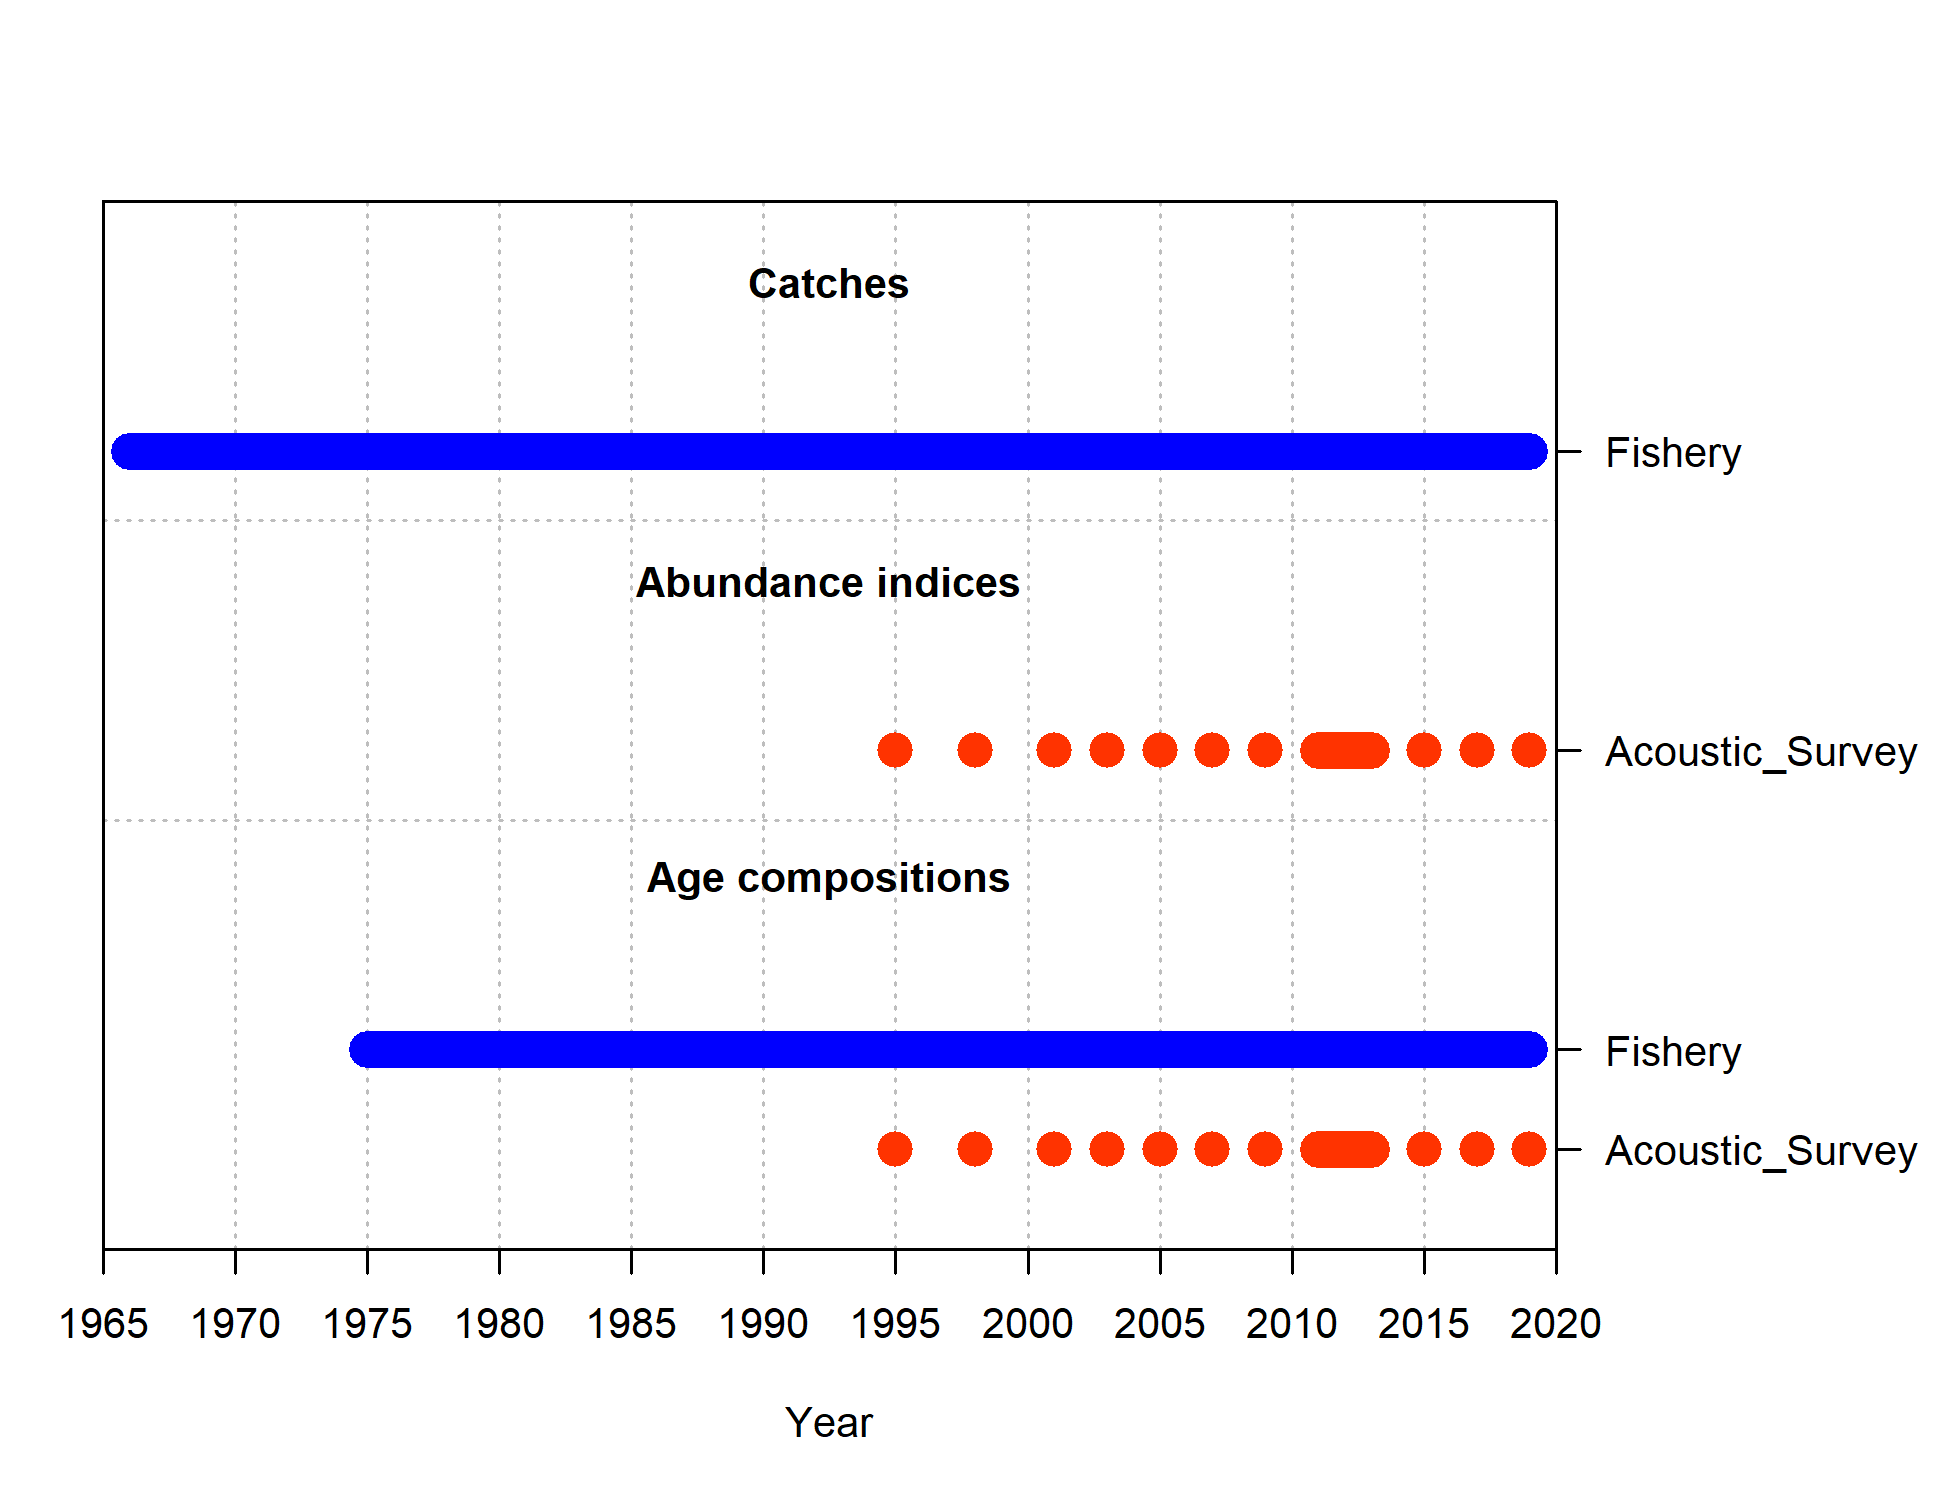
\includegraphics[width=1\textwidth,height=1\textheight]{data-plot.png}
\caption{Summary of data sources used in the base model.\label{fig:data-plot}}
\end{figure}
\end{document}
